%
%  Copyright © 2022 Mateusz Stompór. All rights reserved.
%

\chapter{Przegląd dostępnych rozwiązań}
\section*{Wprowadzenie}
Rozumiejąc główne koncepcje stojące za generowaniem grafiki trójwymiarowej możliwe jest dalsze zgłębienie gałęzki informatyki odnoszącej się do tego zagadnienia.
Na przestrzeni lat powstał niemały zasób literatury poruszający tematykę.
Rozwiązania - silniki - będące implementacją idei rozwinięto do tego stopnia, że same w sobie nie są już komponentami aplikacji, ale wyewoluowały do samodzielnych, pełnoprawnych produktów.
Choć realizowane cele wydają się być identyczne - tworzenie obrazu na podstawie opisu sceny - to podejścia, które stosują różnią się znacząco od siebie.
Podobnie odmienne są wykorzystywane technologie.
Dotytyczy to zarówno programowania samej aplikacji, jak i komunikacji z GPU.
Celem niniejszego rozdziału będzie przegląd rozwiązań dostępnych na rynku, zestawienie ich ze sobą i analiza możliwości platform ekosystemu Apple.
\section{Materiały źródłowe}
Mając na uwadze współczesne trendy - potęgowanie informacji na skutek globalizacji i faktu iż każdy jest w stanie stworzyć publikacje - nie sam dostęp do informacji stanowi problem, a wartościowość źródeł.
Dokonująć przeglądu dostępnej literatury wyraźnie dostrzec można, że szczególną popularnością wśród obiorców cieszą się książki.
Ponadto, równie dużym zainteresowaniem i wkładem w rozwój dziedziny pochwalić mogą się publikacje pracowników firm z branży filmowej oraz gier.
Nie są to jednak jedyne kanały dostępne dla współczesnego odbiorcy.
Ostatnie piętnastolecie zaowocowało intensywnym rozwojem platform streamingowych.
Możliwość ta nie tylko pozwoliła zaangażować się twórcom niezaleznym, ale włączyła także instytucje, takie jak uczelnie.
Zainteresowani mogą bezpłatnie skorzystać z nagrań cyklów wykładów, które niegdyś zarezerwowany były tylko dla nielicznych.
\par
Źródła dostępne w formie książek podzielić można na kilka głównych kategorii - jest to literatura poświęcona odpowiednio: matematyce w świecie grafiki oraz implementacji algorytmów, śledzeniu promieni, a także projektowaniu i budowie silników do gier.
Nie można zapomnieć o narzędziach które konieczne są do rozwoju technologii - w tym kontekście odnosi się to do języków programowania w których technologie są tworzone - API programistycznych oraz środowisk na których są uruchamiane, takich jak systemy macOS, iOS, Windows, Linux.
\par
Pierwszą groupę, rozważającą aparat matematyczny oraz algorytmy wykorzystywane w generowaniu grafiki, reprezentują takie tytuły jak \textit{3D Math Primer for Graphics and Game Development}~\cite{math_f_dunn_i_parberry}, \textit{Real-Time Rendering}~\cite{real_time_rendering}.
Dostępne są one od wielu lat, posiadają szereg wydań i nieprzerwanie górują w wynikach sprzedaży na platformach takich jak eBay czy Amazon.
Choć statystyki sprzedaży nie muszą wiązać się z jakością samego dzieła to wartość wspomnianych tytułów podparta jest mnogimi referencjami w bibliografiach publikacji naukowych.
Obie pozycje skierowane są do osób posiadających niewielkie zaplecze inżynieryjne i stworzone przy założeniu, że czytelnik dopiero rozpoczyna zgłębianie tematyki.
Oba z dzieł przybliżają nomenklaturę używaną w branży, koncepcje przyjęte powrzechnie, opisują aparat matematyczny by w końcu przejść do właściwej części jaką jest renerowanie grafiki.
Mając szerszy ogląd nie sposób przeoczyć fakt, że pomimo ciągłej pracy ze strony autorów nie jest to odpowiednia literatura dla odbiorców poszukujących najświeższych nowinek.
Bezsprzecznie zagwarantować mogą silne podstawy i nakreślić idee, jednak chcąc stworzyć technologie aktualną należy odwołać się także do alternatyw.
\par
Warto pamiętać również o literaturze poruszającej kwestie rzucania promieni. 
Można przytoczyć tutaj między innymi \textit{Ray Tracing Gems}~\cite{ray_tracing_gems} oraz \textit{An Introduction to Ray Tracing}~\cite{ray_tracing_introduction}.
Zakres, który opisują jest znacznie szerszy niż współcześnie można wykorzystać w silniku czasu rzeczywistego, natomiast wiedza, która jest tam zawarta jest konieczna do uzyskania rozwiązania hybrydowego.
W szczególności tyczy się to algorytmów generowania odbić światła (refleksji), rzucania cienia czy okluzji ambientowej.
\par
Zrozumienie zasad generowania grafiki nie jest jednak wystarczająca do stworzenia biblioteki graficznej, ani bardziej obszernego wcielenia - silnika gry.
W tym celu należy zapoznać się z architekturą owocy branży rozrywkowej\cite{game_programming_patterns}.
Na rynku dostępne są produkcje stworzone wprost przez pracowników takich studiów jak \textit{Naughty Dog}\cite{game_engine_architecture} czy \textit{Electornic Arts}\cite{game_programming_patterns} opisujące problemy jakie twórcy mogą doświadczyć oraz propozycje ich rozwiązania.
Stonowi to nieodłączny suplement, ponieważ biblioteki graficzne czy też silniki gry mają za zadanie wyabstrahować skomplikowane techniki renderowania i zapewnić użytkownikowi środowisku w którym będzie w stanie realizować wizję artystyczną bez konieczności rozumienia detali implementacyjnych.
Jeśli chodzi o sam interfejs programistyczny trudno wytypować konkretne tytuły mogące pomóc w procesie projektowania.
Odwołać należy się do ogólnie przyjętych \q{dobrych} praktyk programistycznych, co w tym kontekście oznaczać może przejrzysty interfejs i możliwie wysoką hermetyzację.
\par 
Kolejnym ważnym elementem są źródła, które pozwalają przekuć idee związaniem z generowaniem grafiki w program komputerowy.
Z racji na platformę, oczekiwanie wysokiej wydajności wybór ogranicza się do języków takich jak Swift, Objective-C - natywnych dla macOS - oraz C++.
W przypadku C++ oraz Swift liczyć można na literaturę wprost od autorów \cite{cpp_bjorne}\cite{swift_docs}.
Objective-C choć stale wspierany i używany powszechnie nie jest już rozwijany i wachlarz dostępnych pozycji jest ograniczony. 
Pomimo tego pewne z nich zdecydowanie można uznać za solidne \cite{objective_c_kochan}. 
\par
Wbrew intuicji w przypadku grafiki komputerowej badania publikowane przez uczelnie wyższe rzadko charakteryzują się innowacyjnością.
Zdecydowanie największy wkład we współczesny rozwój mają publikacje firm zaangażowanych bezpośrednio w dziedzinę z przyczyn komerycjnych.
Organizacje takie jak Crytek, Electronic Arts, Epic Games czy Ubisoft chętnie dzielą się informacjami związanymi z technikami renderowania i modelami oświetlenia.
Przykładami mogą być modele oświetlenia w silnikach \textit{Unreal Engine}~\cite{real_shading_ue_4} czy \textit{Frostbite}~\cite{moving_frostbite_to_pbr}.
Nie brakuje także przełomowych algorytmów, takich jak powszechnie używane \textit{SSAO}~\cite{finding_next_gen_cryengine2} stworzone przez Crytek czy \textit{mgła wolumetryczna}~\cite{volumetric_fog} przez Ubisoft.
Niezaprzeczalnie jednak w procesie tym przewodzą giganty takie jak Pixar czy Disney.
Nie tylko opisują oni jakie metody stosują, ale także tworzą sprawozdania podumowujące prace związane z konkretnymi produkcjami, ale także upubliczniają własne modele scen do mierzenia wydajności.
Zgodnie z tym co wspomniano na początku - wiedza z branży filmowej nie przkłada się bezpośrednio na ogólnie pojęte renderowanie czasu rzeczywistego - to jednak w obliczu układów tworzonych współcześnie - wyposażonych w moduły akceleracji raytracingu - podejście to zyskuje na użyteczności.
\par
W ostatniej grupie źródeł - dystrybuowanych w formie materiałów wideo - umieścić można cykle wykładów z uczlni \textit{UC Davis}~\cite{uc_davis_computer_graphics}, \textit{MIT}~\cite{mit_computer_graphics} oraz \textit{Indian Institute of Technology Delhi}~\cite{iiotd_computer_graphics}. 
Są to kursy poruszające ogólną tematykę generowania obrazu.
Najaktualniejszy spośród nich należy do MIT - wykłady publikowane są corocznie.
Zrealizowane są one kompleksowo - zagadnienia są omówione szczegółowo, a w przypadku gdy wykraczają one poza przewidziany materiał prelegent informuje z jakiego zakresu należy wiedzę tę rozszerzyć.
Odbiorca więc nie będzie mógł posiąść wiedzy kompletnej na podstawie wideo, ale będzie wiedział jakie kierunki powinien zgłębić.
Pozostałe dwa kursy pomimo upłynięcia wielu lat od publikacji nadal są przydatne.
W szczególności \textit{Ken Joy} w ramach pracy w UC Davis opisuje dokładnie algorytmy wykorzystywane w sprzętowej akceleracji grafiki komputerowej.
Nie jest to wiedza niezbędna dla osoby chcącej zbudować silnik, ale pozwala zrozumieć w pełniej skali jak wygląda przebieg rasteryzacji.
\par
Równie użyteczne są wystąpienia pojedynczych osób - pracowników z branży gier - którzy opowiadają o podejściu, jakie należy stosować w celu uzyskania aplikacji o optymalnej wydajności.
Z uwagi na formę - zwykle jest to pojedynczy wykład nieprzekraczający godziny czasu - są one zwięzłe i jedynie nakreślają kierunek, jednak z racji iż branża gier potrzebuje najwyższej klasy wydajności to wzorce projektowe i podejście do programowania aplikacji niejednokrotnie budzi kontrowersje.
Podpierając opinie przykładem można tutaj odwołać się do dwóch nagrań z konwencji \textit{CppCon}, które górują w listach popularności.
Mowa tutaj o \eng{Data Oriented Design} przedstawione przez Mike'a Actona~\cite{mike_acton_dod} oraz Stoyana Nikoleva~\cite{stoyan_nikolov_dod}.
\par 
W przypadku platform Apple źródłem, które nie może być pominięte są wydarzenia WWDC~\cite{wwdc_conferences}.
Ich siłą jest możliwość zapoznania się z nowinkami technologicznymi, jakie twórcy udostępniają dla użytkowników swojego sprzętu.
Dodatkowo, często stanowią też okazję do skorygowania podejścia używanego przez programistów w celu zapewnienia optymalnej wydajności.
Przybierając przy tym formę zwięzłej prezentacji 20-60 minut wraz z dostarczeniem kodu źródłowego do samodzielnej analizy.
\par 
Ostatnimi, wartymi do przywołania źródłami są kanały w platformie youtube twórców niezależnych i pracowników korporacji zajmujących się produkcją gier.
Głównie wynika to z faktu, że pierwsi z nich są wyjątkowo otwarci na komentarz dotyczący technologii, które zastosowali i opisania krok, po kroku jak wygląda logika działania ich aplikacji.
Drudzy natomiast chętnie w formie dialogu z widzami przeprowadzają code-review lub też rozwijają wątki związane z tworzeniem silników.
Siła tej formy przekazu wynika z interaktywności.
Filmy same w sobie nie posiadają ograniczenia czasowego, nagrywający nie ponosi kosztów związanych z produkcją, ponieważ są one amatorskie, a sami widzowie mogą zadawać pytania, które adresowane mogą być w krótkim czasie.
Wśród wielu twórców przywołać można kanały takie jak ThinMatrix~\cite{yt_thin_matrix} czy TheCherno~\cite{yt_the_cherno} ponieważ są one nadwyraz rozpoznawalne wśród entuzjastów grafiki komputerowej.
\par
Podsumowując, globalizacja, otwartość uczelni, a także korporacji sprawia, że dostęp do wartościowych informacji nie stanowi żadnego problemu.
Dziedzina obfituje w wysokiej jakości źródła i wydaje się, że stworzenie rozwiązania bazującego na współczesnych trendach nie powinno stanowić wyzwania.
Problemem będzie natomiast nakład pracy potrzebny do uzyskania dzieła kompletnego pod względem funkcjonalnym oraz dobór technologii.
\section{Silniki 3D}
Mnogość źródeł jednoznacznie wskazuje, że gałąź jest dojrzała i oczekiwać można równie obfitej puli dostępnych rozwiązań.
Jest to w pełni prawidłowe założenie.
Rynek jest na tyle obszerny, że początkowo trudno zorientować się kto stanowi grono odbiorców dla poszczególnych produktów.
Poniższa sekcja ma na celu przybliżenie rozwiązania tego problemu.
\par
W celu dokonania klasyfikacji konieczne będzie przygotowanie listy charakterystyk na podstawie których przykłady zostaną porównane.
Wśród wielu możliwych do najważniejszych zaklasyfikować możemy cechy produktu stanowiące odpowiedzi na pytanie takie jak:
\vspace{-0.5\topsep}
\begin{itemize}
    \setlength{\parskip}{5pt plus 0pt}
    \setlength{\itemsep}{5pt plus 5pt}
    \item Czy jest multiplatformowy?
    \item Na zasadach jakiej licencji jest dystrybuowany?
    \item Czy jest aktywnie rozwijany?
    \item Czy dostępna jest dokumentacja i przykłady wykorzystania?
    \item Czy kod źródłowy jest otwarty?
    \item Jakie przypadki użycia realizuje?
    \item Jak wygląda kwestia rozszerzalności?
\end{itemize}
\vspace{-0.5\topsep}
Znalezienie odpowiedzi pozwoli oszacować, które obszary branży pokryte są przez istniejące rozwiązania.
Dodatkowo, umożliwi dostrzeżenie nie tylko silnych stron, ale także nisz, które kryją w sobie potencjał i mogłyby skorzystać z ulepszeń.
\subsection{Biblioteki multiplatformowe}
Jedną z dwóch możliwości dystrybucji oprogramowania jest forma multiplatformowa.
W założeniu polega ona stworzeniu jednego rozwiązania dostępnego na co najmniej dwóch platformach.
Warto podkreślić, że chodzi tutaj o architekturę w której istnieje część wspólna - w rozpatrywanym znaczeniu nie należy uwzględniać oprogramowania realizującego identyczne funkcje, ale za pomocą ponownej implementacji przy użyciu natywnych technologii.
Obszar współdzielony tworzony jest w technologi dostępnej na każdej ze wspieranych platform.
Dodatkowo, ponad warstwą centralną znajduje się wartwa specyficzna dla platformy.
Ma ona za zadanie oddać do użytku oprogramowanie uwzględniając różnice wynikające z innego systemu operacyjnego, a także technologii.
Przykładowo programista systemu Android oczekiwał będzie API w formie biblioteki JAVA lub Kotlin, zaś twórca aplikacji iOS powinien mieć dostęp za pośrednictwem języków Swift czy Objective-C.
\begin{figure}
    \begin{center}
        \includegraphics[width=10cm]{images/multiplatform-architecture.png}
    \end{center}
    \caption{Demonstracja idei oprogramowania mulitplatformowego}
    \label{fig:multiplatform}
\end{figure}
\par
Głównym argumentem stojącym za budowaniem oprogramowania w sposób multiplatformowy jest chęć zwiększenia grona odbiorców.
Dla konsumenta technologii jest to niewątpliwa zaleta, natomiast narzuca to na twórców dodatkową prace związaną z koniecznością uwzględnienia wpływu zmiany na wszystkie dostępne warianty.
Dodatkowo, konieczność wprowadzenia generalizacji wiąże się z narzutem związanym z wydajnością. 
Kolejnym aspektem, który należy wziąć pod uwagę jest sposób i jakość integracji z natywnym środowiskiem.
Chodzi tutaj o kwestię czy interfejs biblioteki dla końcowej platformy uwzględnia konwencje na niej stosowane i jak łatwe możliwe jest jego zintegrowanie.
\subsubsection{Unity}
Najpopularniejszym silnikiem grafiki trójwymiarowej na platformie iOS jest Unity.
Stworzony został z myślą o produkcji gier wideo.
Dostępny jest na większości platform, zarówno mobilnych, jak i stacjonarnych, ale w głównej mierze przeznaczony jest do mniejszych projektów.
\par
Rozwiązanie należy zaliczyć do płatnych, choć rozwój aplikacji wykorzystującej technologię można rozpocząć bezpłatnie.
Użytkownik, który jednak poważnie myśli o wydaniu komercyjnie rentownej aplikacji szybko dostrzeże mnogość ograniczeń.
Do najpoważniejszych zaliczyć można brak możliwości zmiany ekranu ładowania aplikacji czy niemożność dostępu do kodu aplikacji silnika.
\par
Z drugiej strony Unity to twór kompletny - pozwala na tworzenie w technologiach 2D, 3D, VR oraz AR.
Posiada zintegrowane moduły do obsługi fizyki, dźwięku, kontrolerów, analityki użycia, a także reklam.
\par
Choć od strony funkcjonalnej rozwijany jest w języku C++ to użytkownik dokonuje interakcji za pomocą C\#.
W założeniach chodzi o to, aby silnik skompilować tylko raz, a każda modyfikacja, której użytkownik chce dokonać w rozgrywce gry jest błyskawiczna.
Mono - framework wykorzystywany przez Unity w tym celu - ma jednak pewne mankamenty.
Przede wszystkim użytkownicy narzekają na okazjonalne przycięcia w grach wynikające ze sposobem zarządzania pamięci przez technologię.
Dziwić może także sama obecność C\#.
Unity deklaruje, że najlepiej odnajduje się na mobilnych platformach, ale język skryptowy nie pokrywa się z żadną wiodącą technologią ze świata smartfonów.
Na obronę jednak przyznać należy, że grę w unity można stworzyć bez znajomości platformy docelowej.
\par
Dodatkowo, Unity jest rozszerzalne. 
Dokonać można tego za pomocą pluginów występujących w dwóch formach.
Jest to odpowiednio plugin natywny dla zadanego systemu operacyjnego, albo zgeneralizowany oferujący zgeneralizowaną funkcjonalność.
\par
Pomimo faktu, że Unity jest stale rozwijane to brakuje grafika wydaje się odstawać od konkurencji.
Podkreślić należy, że potok renderowania silnika jest konfigurowalny, więc jeśli grafika dla odbiorcy jest niezadowalający istnieje możliwość dokonania korekcji we własnym zakresie.
Otwiera to także możliwość stworzenia zupełnie unikalnego stylu graficznego.
Unity choć opiera się o PBR to za pomocą własnych programów cieniujących istnieje możliwośc nadania własnego charakteru.
\par
Sama dokumentacja projektu stoi na wysokim poziomie.
Obfita jest w liczne przykładowe projekty i zawiera sugestie co do sposobu implementacji pewnych funkcjonalności w sposób zgodny z pierwotną wizją autorów.
\par
Pierwotnie cała interakcja warstwy gry oraz silnika obsługiwana była za pomocą skryptów C\#.
Na przestrzeni lat rozwinięto jednak interfejs graficzny środowiska, a także dodano możliwość konfigurowania przebiegu rozgrywki za pomocą programowania wizualnego.
W założeniu podobne jest to nieco do schematów blokowych używanych w celu objaśniania algorytmów.
Koncept miał za zadanie otworzyć silnik na szersze grono odbiorców i zaoferować możliwośc tworzenia gier osobom nie będącym znajomym z programowaniem.
Choć pomysł może wydawać się oszczędzać czas i ułatwiać rozwój to wiele osób nadal niechętnie korzysta z rozwiązania.
W głównej mierze podyktowane jest to bardzo kiepską przejrzystością zmian dokonanych przez użytkowników w systemach kontroli wersji.
Równie często przywoływany jest także argument wskazujący na trudność w odnajdywaniu się w logice stworzonej przy pomocy programowania wizualnego.
Równoważna implementacja w formie skryptu przywoływana jest jako bardziej przejrzysta i łatwiejsza do objęcia zrozumieniem.
\par
Za minus można uznać też narzut w kwestii wagi aplikacji.
Szablon pustego projektu wiąże się z koniecznością posiadania około 20 MB wolnej przestrzeni.
Natywny, pusty projekt iOS to zaledwie około 1 MB.
Wydawać może się, że to niestotne, jednak z uwagi na fakt, że aplikacje mobilne często pobierane są za pomocą transmisji komórkowej, a na jej efektywność wpływa wiele czynników, to naturalnie narzut wagi powinien być ograniczony do minimum.

% Unity is all but tailor-made for mobile
% requires optimization, takes lots of space
% lots of poor performance assets
% Not so good visuals
% Lack of support for networking
% Uses mono for scripting, so engine is in c++ but scripting in c#
% performance issues related to mono
% closed source - access is possible but fees are great 
\begin{figure}
    \begin{center}
        \includegraphics[width=10cm]{images/engines/unity/example-game.png}
    \end{center}
    \caption{Przykładowa gra stworzona w silniku Unity}
    \label{fig:unity-example-game}
\end{figure}

% \subsubsection{Godot}
% Reprezentuje wszystko za pomocą grafu sceny
% Posiada UI do tworzenia gry - node'y, animacje
% Napisać, że jak chcemy interfejsować z silnikiem to trzeba pisać pluginy do godota
% Posiada visual scripting za pomocą bloków
% używa GDScript do skryptowania, można skryptowac C sharp albo C++
% Napisać, że obecnie jest w wersji 4
% Napisać, że godot jest właściwie vulkan only
% działa na macos i apple silicon od wersji 3.3 - ale wtedy opierało się to na opengl
% teraz gdy apple odeszło od opengl godot kompiluje swoje shadery z vulkan do metal
% Na ten moment nie jest to stabilne
% community driven
% https://godotengine.org/showcase
% https://itch.io/games/made-with-godot/platform-ios
% Napisz, że gier na iosa to w sumie jest mało
% \begin{figure}[H]
%     \begin{center}
%         \includegraphics[width=15cm]{images/engines/godot/editor.png}
%     \end{center}
%     \caption{Edytor treści w silniku Godot}
%     \label{fig:godot-editor}
% \end{figure}

% \subsubsection{Unreal Engine}
% low end devices
% small teams
% open source
% 5 procent od sprzedaży unita powyżej pewnej sumy gross
% good performance
% May be overwhelming for a single person
% Constant patches
% Visual programming may be difficult and less visible for merges
% Inefficient use of data

% " UE4 is not intended to visualise and manage the sheer number of weapons, armor, consumables, conversations, and so on, needed for an RPG."

% UE4 is well suited to bigger games, so think carefully if you're aiming for a smaller project -- various aspects could run slowly, from the editor itself to official support. Unity may be better suited to your needs if you're working on a small game or a mobile game.

% "UE4 comes with the background of being an engine for large AAA titles supporting tons of features for all kinds of advanced systems," Hazelight's Coulianos says. "Therefore the editor can run slow, and seem a bit overkill if you are making a very small and simple game -- for a phone, for example."

% not very popular in simulation/racing games
% super grafika
% good for large, complex game
% blueprints - visual programming
%  lots of materials for learning
% \fig{images/engines/ue/blueprints.png}{Kreator tworzenia logiki w silniku Unreal Engine 4}{fig:ue-blueprint}

% \begin{figure}[H]
%     \begin{center}
%         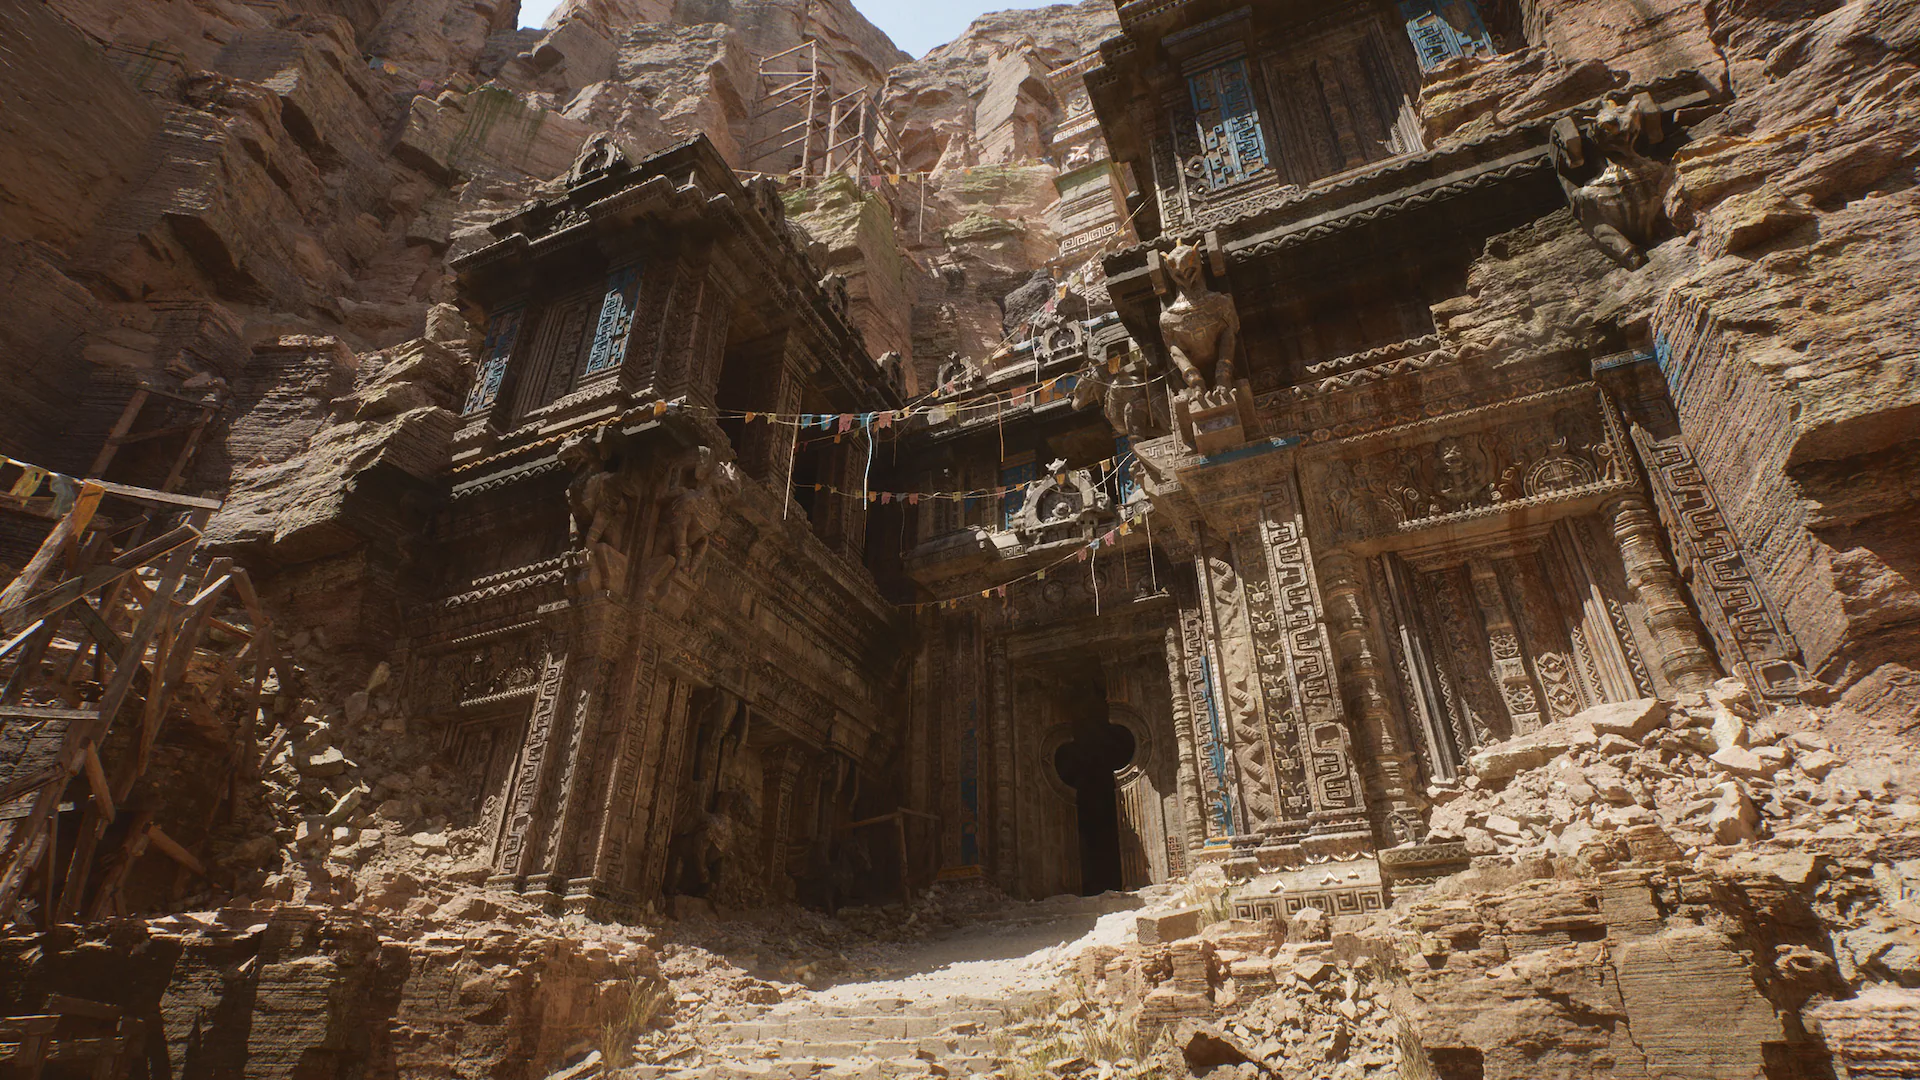
\includegraphics[width=15cm]{images/engines/ue/photorealistic-temple.png}
%     \end{center}
%     \caption{Przykład renderowania hybrydowego w Unreal Engine 5}
%     \label{fig:ue5-photorealistic-temple}
% \end{figure}

% \subsubsection{Filament}
% \begin{figure}[H]
%     \begin{center}
%         \includegraphics[width=7cm]{images/engines/filament/helmet.jpeg}
%     \end{center}
%     \caption{Przykład klatki wygenerowanej przez silnik Filament}
%     \label{fig:filament-helmet}
% \end{figure}

\subsection{Biblioteki natywne}
Alternatywą do multiplatformowych rozwiązań są biblioteki natywne.
Zaliczyć do tej grupy możemy produkty dostępne tylko i wyłącznie na pojedynczej platformie lub te, które dostępne są na wielu, lecz każdy warient zbudowany jest od początku z myślą o platformie.
Pomimo, że wsparcie pojedynczego środowiska stanowi ograniczenie przez wzgląd na dużo mniejszą grupę odbiorców w stosunku do wieloplatformowych odpowiedników to przynosi także korzyści.
Do najwazniejszych zaliczyć możemy możliwośc uzyskania optymalnej wydajności, większą intuicyjność wynikającą z możliwości tworzenia interfejsu dostosowanego do przyjętych konwencji.
Dodatkowo, pozwalają na dostęp do wszystkich funkcjonalności platformy i są łatwiejsze w debugowaniu przez wzląd na fakt, że stworzone są w oparciu o natywne technologie.

\subsubsection{SceneKit}
\begin{figure}
    \begin{center}
        \includegraphics[width=15cm]{images/engines/scene-kit/editor.jpg}
    \end{center}
    \caption{Edytor treści w silniku SceneKit}
    \label{fig:scenekit-editor}
\end{figure}

\begin{figure}
    \begin{center}
        \includegraphics[width=15cm]{images/engines/scene-kit/example-game.jpg}
    \end{center}
    \caption{Przykładowa gra w silniku SceneKit}
    \label{fig:scenekit-example-game}
\end{figure}
Debiut rozwiązania nastąpił w 2012 roku. 
Za projekt i wykonanie odpowiedzialna jest firma Apple, której urządzenia stanowią jedyną decelową grupę odbiorców oprogramowania.
Początkowo wsparcie ograniczało się do platformy OS X, rozszerzenie dostępności na urządzenia mobilne została odroczone do 2014 roku.
Na przestrzeni lat dodano również wsparcie dla watchOS oraz tvOS.
\par
Pragnąc zaklasyfikować SceneKit najtrafniej byłoby określić, iż jest to biblioteka graficzna realizująca dodatkowo pewne funkcjonalności silnika do gier.
Jest to możliwość kontroli audio oraz integracja silnika fizycznego. 
W przeciwieństwie do wiodących rozwiązań skierowanych do branży gier SceneKit nie pozwala na skryptowanie, ani programowanie wizualne.
Niewątpliwą zaletą takiego stanu rzeczy jest znacznie łatwiej użytkownik biblioteki jest w stanie przyswoić sobie możliwości biblioteki.
\par
Myśląc o grupie decelowej wskazać można deweloperów tworzących gry typu indie - w niewielkiej grupie, z małym budżetem.
Ponadto, SceneKit świetnie sprawdza się w roli generatora grafiki trójwymiarowej w aplikacjach innych niż gry wideo.
Z uwagi na fakt, że jest to technologia natywna bardzo łatwo wkomponowac można widoki z animowanymi scenami w aplikacje pełniącą inną funkcje niż rozrywkowa.
Sam narzut w kwestii wielkości paczki również jest niewielki, co tylko potwierdza tezę.
% Kod źródłowy projektu nie jest publiczny, jednak uzyskanie dostępu do plików binarnych biblioteki jest darmowe.
% Nie podlega opłacie także wykorzystanie jej we własnym projekcie bez względu czy jego dalsza dystrubucja jest odpłatna.
\par
Nie bez przyczyny wspomniano o dacie wydania biblioteki.
Choć jej interfejs ewoluował i rozrastał się w miarę upływu lat to założenia pozostały niezmienione.
2015 był rokiem kiedy podczas konferencji WWDC Apple zaprezentowało koncepcje, które sugerują programistom wykorzystującym język Swift.
W głównej mierze ogólnić można je na zestaw sugestii, które sprawią, że kod będzie reużywalny, testowalny oraz przejrzysty.
Je same postanowili także wcielić w swoje biblioteki i w miarę uaktualniania języka Swift i tworzenia nowych bibliotek rozszerzających funkcjonalności iOS Apple stawiało na luźne powiązania pomiędzy komponentami i testowalność.
Niestety reforma ta nie dotknęła SceneKit.
\par
2018 rok był ostatnim kiedy wprowadzono usprawnienia do produktu.
Od tamtego czasu użytkownicy nie otrzymali żadnych poprawek, ani stanowiska Apple wyjaśniającego przyszłość projektu.
Sytuację komplikuje fakt, że kod źródłowy jest zamknięty, więc użytkownicy nie są w stanie na własną rękę skorzystać z nowinek technologicznych.
\par
Pomimo, że Apple jest gigantem, ma ogromne dochody i przez wielu programistów traktowane jest jako miejsce w którym jakość jest najważniejsza to nadal w pewnych kwestiach można poczuć się zawiedzionym.
Jednym w takich chwil jest spojrzenie na dokumentację SceneKit.
Przyznać należy, że w siecie dostępnych jest wiele projektów demonstrujących działanie.
Natomiast pozytywny obraz przyćmiewają wszyechobecne lakoniczne opisy odnoszące się do zawartości biblioteki.
Niejednokrotnie klasy oraz ich zmienne posiadają wyjaśnienia w formie pojedynczych zdań, nie nadających im szerszego kontekstu.
Odnieść można wrażenie, że jedyną drogą do zrozumienia pewnej puli z zaimplementowanych mechanizmów będzie wysnucie własnych wniosków na podstawie empirycznych doświadczeń.
\subsubsection{ARKit}
Wydanie ARKit było odpowiedzią na rosnące zainteresowanie branży technologią rozszerzonej rzeczywistości.
Idea polega na wzbogacanie obrazu przechytywanego z kamery urządzenia o dodatkowe elementy 2D oraz 3D.
Podobnie jak w przypadku SceneKit jest to autorska biblioteka Apple.
Choć część funkcjonalności współdzielona jest z SceneKit to firma deklaruje, iż rozwiązania nie są w żadnym stopniu powiązane ze sobą.
\par
ARKit poprawia wiele problemów, które obecne są w SceneKit.
Przede wszystkim jest ona aktywnie rozwijana, na bieżące publikowane są poprawki, a także rozszerzenia funkcjonalności.
Bibliotekę pochwalić należy za ulepszony model oświetlenia i wydajność.
\par
Interfejs ARKit jest kolejnym czynnikiem zaskakującym pozytywnie.
Dostosowany jest on do współczesnych konwencji firmy i dobrze integruje się z resztą systemu.
Tak jak wspomniano wcześniej interakcje oparte o luźne powiązania pozytywnie wpływają na testowalność kodu wykorzystującego bibliotekę.
\par
Podobnie jednak jak w przypadku innych bibliotek Apple ARKit nie jest otwarta.
Nie istnieje możliwość wglądu do kodu, ani jego modyfikacji, jednak technologia może być w nieodpłatny sposób wykorzystana i przeznaczona do celów komercyjnych.
\begin{figure}
    \begin{center}
        \includegraphics[width=15cm]{images/engines/ar-kit/example-app.jpg}
    \end{center}
    \caption{Rzeczywistość rozszerzona na przykładzie aplikacji mobilnej}
    \label{fig:arkit-example-app}
\end{figure}
\par
Zaskakiwać może również, że w ARKit obsługuje jedynie iOS.
Na pozostałych platformach nie występuje lub tak jak przypadku międzyplatformowej technologii \textit{mac catalyst} wywołania są ignorowane.
Z jednej strony to zrozumiałe, ponieważ tylko telefony i tablety posiadają stosowne kamery spełniające wymagania.
Z drugiej wyklucza to możliwośc wykorzystania ARKit do użycia w celu wygenerowania prostych scen 3D bez AR.
\subsection{Pozostałe silniki}
W celu dokonania rzetelnej oceny rynku dokonano także przeglądu projektów open source udostępnionych za pomocą platform github.com oraz gitlab.com.
Kryterium, którego spełnienia oczekiwano była dostępność na wszystkie platformy Apple i możliwość uruchomienia biblioteki na najnowszych systemach operacyjnych.
W rezultacie wyszukiwania znaleziono wiele projektów, niestety żaden z nich nie mógł określony być jako stabilne rozwiązanie godne do polecenia.
Natywnych dostępnych było poniżej dziesięciu.
Jako te będące w zaawansowanej formie rozwoju wyróżnić można https://github.com/Hi-Rez/Satin czy https://github.com/Hongtae/SwiftVVD.
\par
Warto wspomnieć, że poza wymienionymi przykładami bibliotek oraz silników istnieje wiele innych alternatyw.
Jako najpopularniejsze można przytoczyć tutaj jmonkey, urho3d, OGRE 3D, Amazon Lumberyard czy panda 3d.
Wszystkie z nich oparte są o podejście open-source.
Były to rozwiązania niegdyś popularne lub stale zwiększające swoje zasięgi jednak ze względu na konentracja pracy wokół platform Apple wyłączono je z dalszej analizy.
Głównie za sprawą skierowania jedynie na platformy stacjonarne lub wybrakowane wsparcie spowodowane zamknięciem się firmy Apple na API inne niż Metal.
\par
Sytuacja podobnie wygląda w przypadku produkcji takich jak CryEngine, Frostbite, RAGE czy Naughty Dog Game Engine.
Wszystkie z nich cieszą się niemałą popularnością i sukcesem w świecie gier.
Niestety są one skierowane tylko i wyłącznie na stacjonarne platformy.
Dodatkowo, część podlega opłatą licencyjnym, zaś inne nie mogą być w ogóle użyte z uwagi na fakt, że ich źródła są niepubliczne, a pliki binarne dystrybuowane są jedynie do projektów na potrzeby firmy.
\subsection{Zestawienie}
% Podsumować wszystko
\section{Języki programowania}
Dokonując skrupulatnej analizy należy zastanowić się również nad technologiami, które używane są w popularnych projektach.
Jako podstawą - czynnik fundamentalny - wytypować można język programowania.
Obecnie szacuje się, że liczba dojrzałych wynosi około 300~\cite{programming_languages}.
Pomimo, że grono wszystkich języków jest liczne to tylko kilka z nich używanych jest produkcyjnie w branży gier.
Przesłankami, które najczęściej usłyszeć można jest konieczność uzyskania optymalnej wydajności i wsparcia możliwie dużej liczby platform.
\subsection{C++}
Decyzję o stworzeniu rozszerzenia do języka C, Bjarne Stroustrup - twórca C++ - motywował chęcia otworzenia się na paradygmat programowania obiektowego.
Jego dzieło zachowywało wszystkie dotychczasowe korzyścia wynikające z użycia niskopoziomowego języka, ale sprawiało, że dużo łatwiej programiści byli w stanie tworzyć elastyczne architektury.
Pomimo upłynięcia blisko 40 lat od publikacji pierwszej wersji standardu C++ dowiódł swojej wartości i do dzisiaj jest jednym z najpopularniejszych języków programowania.
\par
Największą siłą, którą w sobie kryje jest mnogość platform na których jest obecny.
Począwszy od telefony komórkowe, samochody, kończąc na branży lotniczej i medycznej.
Użytkownicy - w postaci firm, ale także i osób prywatnych - wskazują, że w głównej mierze chodzi o bezpieczeństwo.
Przez lata kompilatory uzyskały stabilność, a miliony użytkowników pozwalają zachować pewność, nawet w sytuacjach gdzie na szali stoi życie ludzkie.
\par
Długa obecność na rynku niesie za sobą dodatkową wartość.
Pula bibliotek bogata jest w sprawdzone rozwiązania, pokrywające problemy z bardzo wielu dziedzin.
Ponadto, kompatybilność z C sprawia, że szerokie już grono natywnych dla języka bibliotek powiększane jest o te stworzone z myślą o języku C.
\par
Nie jest regułą, że C++ stanowi natywny język dla platformy.
Wręcz to rzadkie zjawisko.
Często programy C++ odpowiedzialne są za wykonywanie tylko i wyłacznie zadań intensywnych obliczeniowo lub ukierunkowanych na niską latencję.
Natomiast same wywołania i odpowiedzi dokonywane są za pośrednictwem języka operującego na wyższym poziomie abstrakcji - takim jak C\#, Java czy Swift.
W razie potrzeby wspomniane interfejsowania może zachodzić także w drugą stronę - z C++ do języka maszynowego.
Możliwość wplatywania C++ w inne technologie niewątpliwie pozwolił utrzymać popularność i uniknąć wyparcia z rynku.
\par
Wreszcie, koncepcją stojącą za stworzeniem języka C była chęć uzyskania technologii będącej w stanie zastąpić język maszynowy, ale zachowując przy tym poziom abstrakcji możliwie jak najniżej.
C++ podtrzymuje to podejście.
W swej istocie oba z nich posiadają proste mechanizmy.
Co za tym idzie mają bardzo niewielki narzut w stosunku do języka maszynowego.
Często, przez wzgląd na wbudowane w kompilator mechanizmy do optymalizacji kod C++ jest lepszy niż równowazny odpowiednik napisany przez człowieka.
\lstinputlisting[language=C++, caption=Przykład kodu w języku C++]{code/example.cpp}
\subsection{Objective-C}
Bjarne Stroustrup nie był jedynym, który dostrzegał braki w języku C i pragnął zmienić stosowane podejście.
We wczesnych latach 80 Tom Love and Brad Cox opracowali własną odpowiedź na ukłon w stronę obiektowości.
Ich dzieło - Objective-C - w pierwszej wersji ukazało się w 1984 roku.
Wybrane zostało przez firmę NeXT jako technologia, którą posłużą się do stworzenia ich autorskiego systemu operacyjnego NeXTSTEP.
Jest on podstawą, którą użyło Apple do rozwijania własnego systemu - znanego dzisiaj pod nazwą macOS - za sprawą przejęcia firmy NeXT w 1996 roku.
\par
W przeciwieństwie do C++ Objective-C nie zyskało tak licznego grona odbiorców jak C++.
Głównie za sprawą faktu, że w głównej mierze prawa do technologii spoczywały w rękach Apple.
W efekcie jest to technologia nadal szeroko-stosowana na ich własnych środowiskach, ale wybrakowana i niemalże nieobecna na innych.
Użycie i wybór Objective-C często podyktowany był koniecznością, a nie rozważną decyzją podpartą argumentami.
\par
Choć język realizuje swoją funkcje to w stosunku do C++ charakteryzuje się gorszą wydajnością.
Wynika to z faktu, że zastosowana tutaj podejście zaczerpnięte ze SmallTalka - wywołanie funkcji za pośrednictwem przesyłania wiadomości do obiektu z nazwą w postaci łańcucha znakowego i listą argumentów.
W tym calu C++ wykorzystuje tablice funkcji wirtualnych, które do wywołania metody wymagają wykonania mniejszej liczby operacji lub niekiedy mogą być całkowicie pomijane.
\par
Dodatkowo, Objective-C zniechęca do siebie swoją składnią, niespotykaną w żadnym innym języku.
Wywołania metod przypominają nieco język naturalny.
W przeciwieństwie do C czy C++ każdy parametr opatrzony jest stosowną nazwą.
Programista w teorii powinien być lepiej zrozumieć działanie algorytmu jednak podejście takie ma także negatywne skutki.
Przede wszystkim wywołania metod są długie, a konieczność zamykania każdego wywołania w nawiasy kwadratowe sprawia, że niekiedy sekwencja wywołań zabiera wiele linii.
\lstinputlisting[language={[Objective]C}, caption=Przykład kodu w języku Objective-C]{code/example.m}
\subsection{Swift}
Debiut Swift nastąpił w 2014 roku.
W przeciwieństwie do wcześniej wymienionych języków Swift nie jest ukierunkowany w pojedynczy paradygmat programowania.
Wykorzystywany może być do podejścia zorientowanego obiektowo, interfejsowo, a także programowania proceduralnego i funkcyjnego.
Decyzja o jego stworzeniu i inwestycja w technologie była inicjatywą Apple.
Jego kluczowe cechy były bezpośrednią odpowiedzią na zarzuty w stosunku do bolączek Objective-C.
\par
Przede wszystkim krótko bo premierze technologii - w 2015 - roku zdecydowano o konwersji projektu do formy open source.
Projekt przeniesiony został na platformę GitHub wraz z bibliotekami standardowymi.
Od tamtej pory producent aktywnie zachęca do zaangażowania się za pośrednictwem formularza zgłaszania błędów, propozycji rozwoju czy bezpośrednich kontrybucji.
W efekcie Swift obecny także na systemach Linux oraz Windows, a przypadek użycia zawiera nie tylko tworzenie aplikacji dla urządzeń Apple, ale język traktowany jest jako rozsądna propozycja do użycia jako technologia serwerowa.
Apple chciało zerwać z dotychczasowym wizerunkiem, który obecny był w Objective-C.
Użytkownicy dostrzegali, że platforma producenta jest jedyną w której technologia ma zastosowania.
Strategia sprawdziła się.
w 2020 roku -  - szacowano, że Swift jest trzykrotnie częściej wykorzystywany niż swój starszy brat.
% https://www.ideamotive.co/blog/swift-vs-objective-c-which-should-you-pick-for-your-next-ios-mobile-app
\par
Sytuacją, którą traktować można jako punkt zapalny do sworzenia języka była premiera pierwszego iPhone'a w 2007 roku.
Urządzenie odniosło ogromny sukces, a każdy kolejny model pomimo stale rosnącej produkcji wciąż nie był w stanie wysycić potrzeb rynku.
Wraz z rewolucyjnym telefonem producent zaoferował światu coś jeszcze.
AppStore był sklepem dostępnym z poziomu urządzenia za pośrednictem, którego użytkownicy mogli dodawać kolejne aplikacje.
Twórcą mógł byc nie tylko sam producent, ale w zasadzie każdy.
Pojawiał się jednak problem.
Potencjalny deweloper musiał nie tylko zaopatrzyć się w telefon, ale także odpowiedni komputer, a dodatkowo nauczyć języka niespotykanego w żadnym innym środowisku.
Apple dostrzegło, że ich trudności odstrasza programistów i w efekcie projekt pomimo doskonałej rentowności nie jest w stanie dojść do swojego szczytu możliwości, w efekcie czego wiele potencjału jest niewykorzystane.
\par
Jedna z kluczowych zalet języka jest prędkość.
Statystyki, poświadczone przez twórców wskazują na 2.6x wzrost wydajności w stosunku do pierwotnego rozwiązania.
Swift nie jest tak dobry jak C czy C++, nie mniej jednak jego narzut jest niewielki.
% https://www.cometchat.com/blog/ios-swift-objective-c-comparison
\par
Nie można przeoczyć także faktu, że nowy język jest czytelny.
W tym znaczeniu można jednak rozpatrywać łatwość w rozumieniu jako ekspresyjność języka.
Aplikacje napisane w Swift są bardziej zwięzłe, obniżając przy tym wymaganą od czytelnika złożoność poznawczą.
\par
Forma licencji i expresyjność języka to nie jedyne czynniki, które za pomocą poprawy miały wpłynąć na przystępność.
W przeciwieństwie do C czy C++ Objective-C nie posiadał jawnie publikowanych standardów, pomimo faktu iż był rozwijany i wersjonowany.
O nowych funkcjach użytkownicy dowiadywali się wraz z dystrubycją nowszych wersji kompilatora.
Nie pomagał fakt, że dokumentacja na stronie Apple opisująca języka opóźniona była o wiele miesięcy, dostępna tylko w jednym języku i napisana bardzo technicznie, bez przykładów.
Swift naprawia ten błąd.
Wraz z premierą twórcy opublikowali książkę w formie elektronicznej \textit{The Swift Programming Language}.
Zakładała ona, że programista nie posiada doświadczenia i stopniowo wdrażała go w coraz bardziej złożone detale języka.
Na pochwałę zasługuje również fakt, że dostępne są liczne translacje, a sam e-book jest darmowy.
Stwarza to wyraźny kontrast w stosunku to słabo opisanego Objective-C z małą ilością źródeł, dostępnych w głównej mierze tylko i wyłącznie po angielsku.
\par
Wydaje się jednak, że Objective-C nigdy nie opuści ekosystemu Apple.
Producent nabiera wody w usta ilekroć temat jest poruszany, ale widoczne są przesłanki na podstawie których sądzić można, że wspomniana teza okaże się prawdziwa.
Tak jak wyjaśniono w stosunku do języka C++ nadal istnieją scenariusze w których odczuć można wyraźna korzyść z oparcia technologii o niskopoziomowe programowanie.
Jeśli taka potrzeba zajdzie w ramach ekosystemu Apple użycie Objective-C jest jedyną drogą dzięki której połączyć można C++ oraz Swift.
\lstinputlisting[language=Swift, caption=Przykład kodu w języku Swift]{code/example.swift}
\begin{figure}
    \begin{center}
        \includegraphics[width=15cm]{images/language-interoperability.png}
    \end{center}
    \caption{Schemat łączenia wielu języków na przykładzie platformy iOS}
    \label{fig:language-interoperability}
\end{figure}
\section{Interfejsy programistyczne}
Ostatnim aspektem, który wymaga analizy jest przegląd dostępnych interfejsów programistycznych kart graficznych. 
% napisać o tensor processing i acceleration structures
% Podkreślić to co już zrobiłem - kiedys były fixed, teraz są programowalne
% Napisać, że w sumie zaczęło się od podejścia immediate
% w miarę postępu czasu mamy kolejki
% api starają się oddać to jak działają współczesne karty graficzne
% w sumie to wszystkie są podobne
% można powiedziec, że każde api ma dwie główne częście
% pierwsza z nich służy do wydawania rozkazów, druga to prgramy cieniujące
%  napisać, że w sumie nowe api przerzucają więcej pracy ze sterownika na programiste
\subsection{DirectX, OpenGL, Vulkan}
\subsection{Metal}
% Napisz o % \subsection{Metal-C++}
% https://alain.xyz/blog/comparison-of-modern-graphics-apis